\documentclass[conference]{IEEEtran}
\IEEEoverridecommandlockouts
\usepackage[T1]{fontenc}
\usepackage[utf8]{inputenc}
\usepackage{textcomp}
\usepackage{cite}
\usepackage{amsmath}
\usepackage{graphicx}
\usepackage{booktabs}
\usepackage{tabularx}
\usepackage{listings}
\usepackage{xcolor}
\usepackage[hidelinks]{hyperref}
\lstset{basicstyle=\ttfamily\scriptsize, columns=fullflexible, keepspaces=true,
  frame=tb, aboveskip=4pt, belowskip=4pt, showstringspaces=false,
  commentstyle=\color{gray}, breaklines=true, breakatwhitespace=true}
% Tables are exactly one column wide: the first column wraps, the others size to content.
\newcolumntype{L}{>{\raggedright\arraybackslash}X}
\setlength{\tabcolsep}{6pt}
% No word is split across a line end: hyphenation off, with \sloppy spacing absorbing
% the lines that would otherwise overrun.
\hyphenpenalty=10000
\exhyphenpenalty=10000
\sloppy

\begin{document}

\title{Capture, Not Retrieve:\\ Behavioural Provenance for Agentic AI}

\author{\IEEEauthorblockN{Munyaradzi Zhou}
\IEEEauthorblockA{University of Trento\\ Trento, Italy\\ munyaradzizhou11@gmail.com}
\and
\IEEEauthorblockN{Sandro Fiore}
\IEEEauthorblockA{University of Trento\\ Trento, Italy\\ sandro.fiore@unitn.it}}

\maketitle

% TODO(authors): this abstract was drafted for the typeset version and has not been
% reviewed. Every figure in it is quoted from the body.
\begin{abstract}
Provenance tooling can record what an agentic AI system did; it cannot record why. We argue
that this gap is structural: the facts a decision used may cross a step boundary, but the rule
that combined them into a verdict is a local computation, and no callback, span or post-hoc
query can retrieve what was never captured. We make the argument measurable with a reflexive
multi-agent demonstrator (four operational agents emitting typed W3C PROV about themselves
and two meta agents governing that output) and a deliberately generous callback-level
baseline over the same run. The baseline reconstructs every activity, all 324 relations and
every verdict, and sees 61\% of the facts the operational justifications cite, but none of the
values the agents computed in order to decide. We publish the \texttt{yp:} vocabulary as an
OWL ontology with SHACL shapes, and measure the cost: building the record is inside every
operational agent's run-to-run variance, justifications are 6.5\% of the records' bytes, and
measured CPU energy per session shows no resolvable difference.
\end{abstract}

\begin{IEEEkeywords}
provenance, W3C PROV, agentic AI, explainability, multi-agent systems, SHACL
\end{IEEEkeywords}

\section{Introduction}\label{sec:1}

\noindent Scientific computing infrastructure is acquiring autonomous agents: they summarise runs, judge results and decide what to archive, increasingly without a human in the loop. The provenance community has a mature answer to \emph{what} such a system did. W3C PROV~\cite{provdm} describes activities, entities and the lineage between them, and capturing that lineage automatically is routine. It has almost no answer to \emph{why}. When a storage agent declines to archive a record, an operator, an auditor and, under the EU AI Act~\cite{euaiact}, a regulator need the reason, not the outcome.

\noindent We argue that this gap is \textbf{structural, not a matter of tooling}:

\begin{quote}
The rationale for a decision is a local computation at the moment of decision. A callback fires after the function returns; a span wraps the call; a query reads the store afterwards. Each may see the facts the decision used. None can retrieve the rule that combined them into a verdict, because that rule was never a value anything passed.
\end{quote}

\noindent We call this \textbf{capture, not retrieve}, and make three contributions. \textbf{C1: the argument, measured.} Against a deliberately generous callback-level baseline over the same run, which recovers every activity, relation and verdict, we show that the facts an agent \emph{computed} in order to decide, and the rule that combined them, are unrecoverable. \textbf{C2: a reflexive multi-agent architecture.} Four operational agents emit typed PROV about themselves; two meta agents govern that output, to a depth bounded by design. \textbf{C3: the \texttt{yp:\allowbreak{}} vocabulary}, published as an OWL ontology with SHACL shapes, and an API whose one hand-written call records the decision. We also measure the cost, in time and in energy.

\section{Background and State of the Art}\label{sec:2}

\subsection{Provenance models and capture systems}\label{sec:2.1}

\noindent W3C PROV~\cite{provdm,provo} models provenance as entities, activities and agents linked by a small set of relations; it is deliberately domain-neutral, and says nothing about rationale. Capture systems differ in where they observe. \emph{Script and workflow} tools (noWorkflow~\cite{noworkflow} for Python scripts, YesWorkflow~\cite{yesworkflow} for annotated workflows) recover lineage from code and execution. \emph{System-level} collectors such as SPADE~\cite{spade} and CamFlow~\cite{camflow} capture whole-system provenance from the operating system, CamFlow emitting W3C PROV-JSON directly. \emph{Machine-learning} trackers record runs, parameters and artifacts: MLflow~\cite{mlflow} with its own schema, and the yProv family (yProv4ML~\cite{yprov4ml} for training runs, yProv4WFs for workflows) in W3C PROV. Surveys of the field~\cite{freire2008,herschel2017} classify provenance by \emph{what} it records and \emph{how} it is captured; across all of them, what is recorded is an observable event. Our demonstrator consumes real yProv4ML records, and every system above could, in principle, observe the agents we build. None could observe their reasoning.

\subsection{Agents, and the observability built for them}\label{sec:2.2}

\noindent Agent frameworks interleave reasoning and tool use~\cite{react} and compose agents into multi-agent systems~\cite{autogen,langgraph}. Their runs are observed by a fast-maturing layer: OpenTelemetry's semantic conventions for generative AI~\cite{otelgenai}, and tracing platforms such as OpenLLMetry~\cite{openllmetry}, Langfuse~\cite{langfuse} and LangSmith~\cite{langsmith}, which record prompts, completions, tool calls, latencies and token counts. This layer is built for debugging and cost attribution. It does not model W3C PROV, and the only rationale it can hold is text a model happened to emit. PROV-AGENT~\cite{provagent} is the closest prior work: it extends PROV to agentic workflows and makes agents and their model calls first-class provenance subjects: a richer \emph{what}, with no field for the reason behind a decision.

\subsection{Rationale, explanation and accountability}\label{sec:2.3}

\noindent Interpretability research asks how a model reaches outputs~\cite{doshivelez2017}, and documentation practice, such as model cards~\cite{modelcards} and datasheets~\cite{datasheets}, records how artifacts were made. Two results bear directly on agents. A model's stated chain of thought is not necessarily faithful to the process that produced its answer~\cite{turpin2023,lanham2023}, so text a model emits is weak evidence of the rule an agent applied. And proposals for the oversight of deployed agents call for exactly the per-action visibility (identifiers, activity logs, the basis of decisions) that a provenance record could carry~\cite{chan2024}. Energy is the third concern of the field: reporting it for ML workloads is now expected~\cite{strubell2019,henderson2020}, usually through sampling tools such as CodeCarbon~\cite{codecarbon}, whose limits for short steps we revisit in Section~\ref{sec:5.3}.

\begin{table}[t]
\centering\footnotesize
\caption{The state of the technology. ``Decision rule'' means the reason an agent's code reached its verdict, as opposed to model text that may describe one. Our capture is automatic except for that one field.}\label{tab:1}
\begin{tabularx}{\columnwidth}{Lcccc}
\toprule
Approach & W3C PROV & Automatic & Agent-aware & Decision rule \\
\midrule
Script, workflow and system capture & yes & yes & no & no \\
ML lifecycle trackers & partly & yes & no & no \\
LLM and agent observability & no & yes & yes & no \\
PROV-AGENT & yes & yes & yes & no \\
This work & yes & partly & yes & \textbf{yes} \\
\bottomrule
\end{tabularx}
\end{table}

\noindent \textbf{Our position is to ride the automatic layer rather than compete with it}: consume what it collects, and add the one thing it structurally cannot.

\section{Vocabulary and Instrumentation}\label{sec:3}

\noindent \textbf{The \texttt{yp:\allowbreak{}} vocabulary} is published as an OWL ontology (86 terms) with SHACL~\cite{shacl} shapes (16 named constraints). It emits only terms the system uses, checked in both directions by a test, and uses PROV's own term wherever one exists: all lineage relations are PROV's. It adds two things PROV lacks: a typed decision lifecycle (Receive, Plan, Act, Observe, \textbf{Decide}, Respond, as subclasses of \texttt{prov:\allowbreak{}Activity}) and \texttt{yp:\allowbreak{}justification}, with \texttt{rdfs:\allowbreak{}domain yp:\allowbreak{}DecisionActivity}, beside \texttt{yp:\allowbreak{}verdict} and \texttt{yp:\allowbreak{}escalation\_\allowbreak{}reason}. The shapes declare the standard: every decision is justified and concluded; every step is typed, dated, ended and attributed; every agent decides something; every \texttt{yp:\allowbreak{}pid} carries a \texttt{sha256:\allowbreak{}} hash. An agent's own runtime check is tested against the shapes rather than trusted to match them, which has found four disagreements, each fixed.

\noindent \textbf{Two layers.} \emph{Layer 1, what happened} (activities, timings, model calls, dataflow) follows mechanically from what a framework callback receives, and the ecosystem of Section~\ref{sec:2.2} already collects it. \emph{Layer 2, why} (the verdict and its justification) cannot be automated. The library automates the first and leaves one call hand-written:

\begin{lstlisting}[language=Python]
with tracker.activity("ToolCallActivity", "write the summary") as prov:
    prov.consumes(task)
    summary = llm.complete(ACT_SYSTEM, facts)
    prov.produces("ResponseEntity", summary.text, pid=pointer, derived_from=task)
    prov.note(**summary.provenance())        # model, prompt hash, tokens

tracker.decide(verdict="REVISE",             # the hand-written line
    justification="Figures 4096 and 512 appear in the summary but not in the graph.")
\end{lstlisting}

\noindent \texttt{decide()} raises on a blank justification. Lineage is declared, never inferred, except \texttt{wasInformedBy}, which PROV defines as derivable; an early tracker that inferred derivations from registration order produced 74 confident, wrong edges of 250. Durations come from a monotonic counter: on our host the wall clock advances in 15.6 ms steps, and before this fix 96 of 96 activities recorded zero duration.

\section{The Demonstrator}\label{sec:4}

\noindent A producer replays real yProv4ML records over a NATS bus to four operational agents, which do work and emit typed PROV about themselves; two meta agents consume \emph{that} and emit PROV in turn. There is no agent framework: the agents are bare asyncio daemons, the strongest evidence that the library is not tied to one runtime.

\begin{table}[t]
\centering\footnotesize
\caption{The six agents. All are domain-agnostic: they compute from PROV itself.}\label{tab:2}
\begin{tabularx}{\columnwidth}{lLl}
\toprule
Agent & Work & Verdicts \\
\midrule
CAx Summariser & LLM summary, figures checked against the graph & ACCEPT/REVISE \\
CA2 Metrics & renders a chart of the run & ACCEPT/REVISE \\
CA3 Analytics & five mining algorithms over any PROV graph & OK/ANOMALY \\
CA1 Storage & persists only after consumers used the record & ACCEPT/ESCALATE \\
MC1 Compliance & checks records against the shapes & PASS/FAIL \\
MC3 Audit & rebuilds the who-did-what-when trail & COMPLETE/PARTIAL \\
\bottomrule
\end{tabularx}
\end{table}

\noindent CA1 writes through the store's API, never the bus, which carries only a receipt (a \texttt{yp:\allowbreak{}pid} and a SHA-256). It persists \emph{after} consumption, at a quorum of consumer acknowledgements, with a timeout guard so a crashed consumer cannot lose a record; its \texttt{yp:\allowbreak{}escalation\_\allowbreak{}reason} separates three conditions demanding different responses: \emph{integrity}, \emph{incomplete-input} and \emph{consumption-unconfirmed}. Envelopes on the bus are numbered, and an agent that finds a gap records an \texttt{INCOMPLETE} decision rather than a well-formed record of a truncated input.

\noindent \textbf{Reflexivity is one level deep, by construction.} Meta agents publish to a subject prefix nothing subscribes to, so governance cannot re-trigger itself. Within that bound the meta agents are fully instrumented, and MC1 satisfies the standard it enforces. One container image serves all roles; CI runs both the containerised NATS path and an in-process path and holds each to the same lineage comparison.

\section{Evaluation}\label{sec:5}

\noindent The reference run is two input records through six agents: \textbf{24 PROV documents}, 96 activities, 324 relations (\texttt{experiments/\allowbreak{}audit-reference}). Every figure is regenerated by code from archives frozen from clean commits, with per-file hashes; 246 tests run on Linux and Windows.

\subsection{Conformance}\label{sec:5.1}

\noindent All 24 documents are accepted by the reference \texttt{prov} parser, and all 24 conform to the published shapes under \texttt{pyshacl}~\cite{pyshacl}, an external judge of an external rule. The relation total is the wrong number to quote: 126 relations are observed, 72 derived, 30 declared and 96 are one-per-activity attributions, so the structural claim is 228. Applied to its input, CA3 found real gaps in yProv4ML's records: 8 of 9 activities declare a start and no end.

\subsection{Capture, not retrieve}\label{sec:5.2}

\noindent Strategy A is a callback-level baseline we built ourselves from the \emph{same run}, fed every step event a framework handler receives. It is an upper bound: its events carry the structural facts the explicit instrumentation declared.

\begin{table}[t]
\centering\footnotesize
\caption{Callback baseline (A, with a ten-rule type map) against explicit capture (B).}\label{tab:3}
\begin{tabularx}{\columnwidth}{Lrr}
\toprule
Signal & A & B \\
\midrule
Activities, typed & 96 & 96 \\
Entities, typed & 0 of 54 & 78 of 78 \\
Relations & 324 & 324 \\
Verdicts & 24 & 24 \\
Justifications & 0 & 24 \\
Accepted by the PROV parser & 24 & 24 \\
\bottomrule
\end{tabularx}
\end{table}

\noindent Structure is recoverable, and so are the verdicts, scraped from node labels, which a graph naming its decision node \texttt{decide} would defeat. No justification appears verbatim in the 12,425 characters A observed, but a run-time sentence rarely survives verbatim, so we test facts:

\begin{table}[t]
\centering\footnotesize
\caption{Each justification's facts (figures, hashes, names, roles) searched for in everything A saw. Seeing a fact over-counts knowing it.}\label{tab:4}
\begin{tabularx}{\columnwidth}{Lrrrr}
\toprule
Decisions & Count & Facts & Seen by A & All seen \\
\midrule
Operational & 8 & 49 & 30 (61\%) & 2 \\
Meta & 16 & 16 & 16 (100\%) & 16 \\
\bottomrule
\end{tabularx}
\end{table}

\noindent The 19 facts A never saw are those the agents \emph{computed in order to decide}: a record's byte count, a timing gap and its share of the run, a summary's length, a threshold. Where A saw every fact, it still lacks the rule: CA2's facts were all visible, but not that finding no numeric values sent it to a fallback chart, nor that the fallback is why it said REVISE. Meta-agent justifications restate structure A already has, and are not counted. \textbf{The inputs to a decision may be observable; the rule that combined them is not.}

\begin{figure*}[t]
\centering
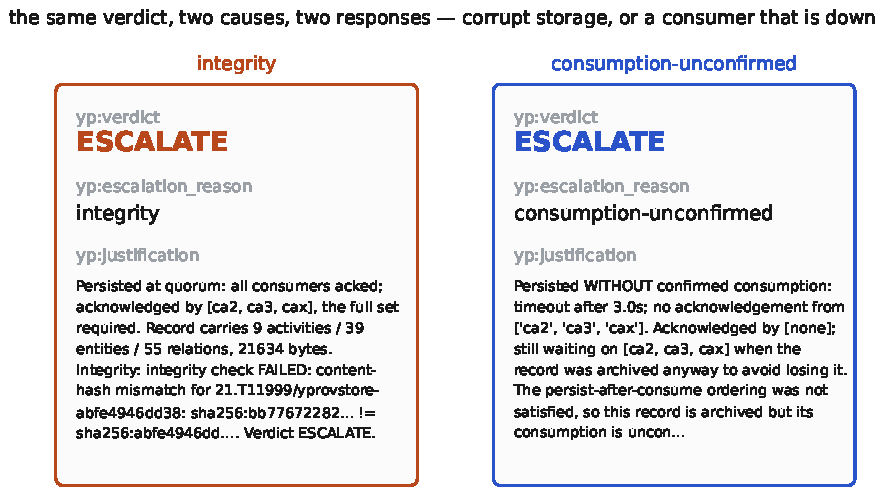
\includegraphics[width=\textwidth]{figures/f4_two_escalations.pdf}
\caption{One verdict, two causes: CA1's integrity and timeout escalations, with both justifications quoted as the record carries them.}\label{fig:1}
\end{figure*}

\noindent Fig.~\ref{fig:1} shows the cost. CA1 says ESCALATE for three reasons; A recovers the verdict, never the reason, so it cannot tell \emph{``storage is corrupting records''} from \emph{``a consumer is down''}.

\subsection{Energy}\label{sec:5.3}

\noindent On our host the CPU is measured (the Windows Energy Meter Interface reads the package counter, tracking load from 5 W idle to 31 W saturated), while memory is a flat 10 W model. A record must say so per component: a sum of the two is labelled \texttt{partly-measured}, never \texttt{measured}. We first concluded the counter was broken; it reads zero until its first sample.

\begin{table}[t]
\centering\footnotesize
\caption{Measured CPU energy per six-agent session, 12 interleaved rounds with idle windows (\texttt{experiments/\allowbreak{}energy-session}). No difference reaches 3x its spread.}\label{tab:5}
\begin{tabularx}{\columnwidth}{Lrrr}
\toprule
CPU energy per session & OFF & B-TRANS & B \\
\midrule
joules & 1.43 & 1.50 & 1.72 \\
vs OFF (margin) & baseline & +5\% (0.9x) & +20\% (2.3x) \\
\bottomrule
\end{tabularx}
\end{table}

\noindent Per step, energy cannot be attributed at all: at a 15 s sampling period a step that did nothing was charged ten times the step that rendered a chart. Each figure therefore carries \texttt{yp:\allowbreak{}energy\_\allowbreak{}sampling\_\allowbreak{}period\_\allowbreak{}s} and \texttt{yp:\allowbreak{}energy\_\allowbreak{}attributable}, and \textbf{energy belongs at session granularity}, where Table~\ref{tab:5} measures it.

\subsection{Model provenance}\label{sec:5.4}

\noindent Every model-bearing step records the model, sampling parameters, prompt identity, version and hash, token counts, latency and a response hash (\texttt{experiments/\allowbreak{}audit-llm}: four calls, 2,071 prompt and 480 completion tokens). The model a caller names is not the one that answers: the record carries the alias \texttt{gpt-4o}, the snapshot \texttt{gpt-4o-2024-08-06} and the provider's fingerprint, and the four calls of one run returned three fingerprints.

\subsection{Overhead}\label{sec:5.5}

\noindent Each agent's step was timed 30 times per condition, interleaved: provenance off, built but not written (B-TRANS), and built and written (B); a difference counts only at 3x its spread. On two occasions, \textbf{building the record was inside every operational agent's run-to-run variance} (margins 0.0 to 0.5x). Writing it resolves for some agents, and there it dominates: for the worst case, MC1, a 109 \textmu{}s step gains 38 \textmu{}s to build the record and 1,485 \textmu{}s to write it (+1,394\%, 98\% of it the write). Transient mode removes 89\% of the time cost; metadata mode 38\% of the bytes, keeping every justification. Recording a justification costs 54 ns against a $\pm$726 ns spread, and justifications are 6.5\% of the records' bytes. Cost is linear (fitted exponents 1.09 and 1.13 to 10,000 activities). Across occasions, two agents' verdicts flipped between resolved and not, so we quote the verdicts that held, the bytes and the complexity class, not the timings.

\subsection{Verdict reachability}\label{sec:5.6}

\noindent The ordinary run reaches six of twelve two-valued verdicts; nine injected scenarios reach the rest, each of CA1's three escalations, and \texttt{INCOMPLETE}: all thirteen are observed. Three scenarios are not faults: CA2 says REVISE on the bundled data because yProv4ML records carry no numeric values, a finding about the input. \texttt{mc1:\allowbreak{}FAIL} is unreachable from this library's own records, because \texttt{decide()} refuses a blank justification; it is reached by a third-party record, which is what a compliance checker is for.

\section{Limitations}\label{sec:6}

\noindent \textbf{We show that justifications exist and that the decision rule is unrecoverable, not that they are good}; whether they improve an operator's decisions needs a human study. The fact-level measure is coarse in both directions. A model-bearing step is repeatable from its record, not reproducible: three fingerprints in one run is a backend changing under a caller that changed nothing. The bus is at-most-once: numbered envelopes expose a partial loss, but a stream lost whole is silent. The evaluation uses two input records, one producer and one machine, and we built the baseline ourselves, mitigated by granting it every declared structural fact.

\section{Conclusion}\label{sec:7}

\noindent Provenance can describe what an agentic system did; with automatic capture alone it cannot describe why, because the rule behind a decision never leaves the agent. We made that measurable against a generous baseline, discharged it with a vocabulary and an API whose one hand-written call records the decision, and found the cost to be storage rather than speed: \emph{storage for explainability, not speed for explainability}. Next: an OpenTelemetry bridge for the automatic half, bounded second-level reflexivity, meta agents that act on their verdicts, and a study of whether justifications improve operators' decisions.

\begin{thebibliography}{30}
\bibitem{provdm} L.~Moreau and P.~Missier, Eds., ``PROV-DM: The PROV data model,'' W3C Recommendation, Apr. 2013.
\bibitem{euaiact} European Parliament and Council, ``Regulation (EU) 2024/1689 laying down harmonised rules on artificial intelligence (Artificial Intelligence Act),'' \emph{Official Journal of the European Union}, 2024.
\bibitem{provo} T.~Lebo, S.~Sahoo, and D.~McGuinness, Eds., ``PROV-O: The PROV ontology,'' W3C Recommendation, Apr. 2013.
\bibitem{noworkflow} J.~F. Pimentel, L.~Murta, V.~Braganholo, and J.~Freire, ``noWorkflow: A tool for collecting, analyzing, and managing provenance from Python scripts,'' \emph{Proc. VLDB Endowment}, vol.~10, no.~12, pp. 1841--1844, 2017.
\bibitem{yesworkflow} T.~McPhillips \emph{et al.}, ``YesWorkflow: A user-oriented, language-independent tool for recovering workflow information from scripts,'' \emph{Int. J. Digital Curation}, vol.~10, no.~1, pp. 298--313, 2015.
\bibitem{spade} A.~Gehani and D.~Tariq, ``SPADE: Support for provenance auditing in distributed environments,'' in \emph{Proc. ACM/IFIP/USENIX Middleware}, 2012, pp. 101--120.
\bibitem{camflow} T.~Pasquier \emph{et al.}, ``Practical whole-system provenance capture,'' in \emph{Proc. ACM Symp. Cloud Computing (SoCC)}, 2017, pp. 405--418.
\bibitem{mlflow} M.~Zaharia \emph{et al.}, ``Accelerating the machine learning lifecycle with MLflow,'' \emph{IEEE Data Eng. Bull.}, vol.~41, no.~4, pp. 39--45, 2018.
\bibitem{yprov4ml} G.~Padovani, V.~Anantharaj, and S.~Fiore, ``yProv4ML: Effortless provenance tracking for machine learning systems,'' arXiv preprint, 2025.  % VERIFY
\bibitem{freire2008} J.~Freire, D.~Koop, E.~Santos, and C.~T. Silva, ``Provenance for computational tasks: A survey,'' \emph{Computing in Science \& Engineering}, vol.~10, no.~3, pp. 11--21, 2008.
\bibitem{herschel2017} M.~Herschel, R.~Diestelk\"{a}mper, and H.~Ben~Lahmar, ``A survey on provenance: What for? What form? What from?'' \emph{The VLDB Journal}, vol.~26, no.~6, pp. 881--906, 2017.
\bibitem{react} S.~Yao \emph{et al.}, ``ReAct: Synergizing reasoning and acting in language models,'' in \emph{Proc. Int. Conf. Learning Representations (ICLR)}, 2023.
\bibitem{autogen} Q.~Wu \emph{et al.}, ``AutoGen: Enabling next-gen LLM applications via multi-agent conversation,'' arXiv:2308.08155, 2023.
\bibitem{langgraph} LangChain, ``LangGraph,'' 2024. [Online]. Available: \url{https://github.com/langchain-ai/langgraph}
\bibitem{otelgenai} OpenTelemetry, ``Semantic conventions for generative AI systems,'' 2025. [Online]. Available: \url{https://opentelemetry.io/docs/specs/semconv/gen-ai/}
\bibitem{openllmetry} Traceloop, ``OpenLLMetry,'' 2025. [Online]. Available: \url{https://github.com/traceloop/openllmetry}
\bibitem{langfuse} Langfuse, ``Langfuse: Open-source LLM engineering platform,'' 2025. [Online]. Available: \url{https://langfuse.com}
\bibitem{langsmith} LangChain, ``LangSmith,'' 2025. [Online]. Available: \url{https://www.langchain.com/langsmith}
\bibitem{provagent} R.~Souza \emph{et al.}, ``PROV-AGENT: Unified provenance for tracking AI agent interactions in agentic workflows,'' arXiv preprint, 2025.  % VERIFY
\bibitem{doshivelez2017} F.~Doshi-Velez and B.~Kim, ``Towards a rigorous science of interpretable machine learning,'' arXiv:1702.08608, 2017.
\bibitem{modelcards} M.~Mitchell \emph{et al.}, ``Model cards for model reporting,'' in \emph{Proc. Conf. Fairness, Accountability, and Transparency (FAT*)}, 2019, pp. 220--229.
\bibitem{datasheets} T.~Gebru \emph{et al.}, ``Datasheets for datasets,'' \emph{Commun. ACM}, vol.~64, no.~12, pp. 86--92, 2021.
\bibitem{turpin2023} M.~Turpin, J.~Michael, E.~Perez, and S.~R. Bowman, ``Language models don't always say what they think: Unfaithful explanations in chain-of-thought prompting,'' in \emph{Advances in Neural Information Processing Systems (NeurIPS)}, 2023.
\bibitem{lanham2023} T.~Lanham \emph{et al.}, ``Measuring faithfulness in chain-of-thought reasoning,'' arXiv:2307.13702, 2023.
\bibitem{chan2024} A.~Chan \emph{et al.}, ``Visibility into AI agents,'' in \emph{Proc. ACM Conf. Fairness, Accountability, and Transparency (FAccT)}, 2024.
\bibitem{strubell2019} E.~Strubell, A.~Ganesh, and A.~McCallum, ``Energy and policy considerations for deep learning in NLP,'' in \emph{Proc. ACL}, 2019, pp. 3645--3650.
\bibitem{henderson2020} P.~Henderson \emph{et al.}, ``Towards the systematic reporting of the energy and carbon footprints of machine learning,'' \emph{J. Mach. Learn. Res.}, vol.~21, no.~248, pp. 1--43, 2020.
\bibitem{codecarbon} CodeCarbon contributors, ``CodeCarbon,'' version 3.3.1, 2025. [Online]. Available: \url{https://github.com/mlco2/codecarbon}  % VERIFY preferred citation
\bibitem{shacl} H.~Knublauch and D.~Kontokostas, Eds., ``Shapes Constraint Language (SHACL),'' W3C Recommendation, Jul. 2017.
\bibitem{pyshacl} RDFLib contributors, ``pySHACL,'' 2025. [Online]. Available: \url{https://github.com/RDFLib/pySHACL}
\end{thebibliography}

\end{document}
